\problemname{Timing}
%{Matthias Bayerlein}{1}

A clash of galaxies is coming!

A galaxy ruled by the mysterious MdI is trying to annex our milky way, but
the galactical government has plans to turn things round.

Our intelligence agency has infiltrated the enemy's headquarter and gained
surprising intelligence. The enemy is moving its units around according to
a fixed scheme: for each fort a fraction of the units is moved to other
forts in each time unit (the time of the flight is negligible).

Now the government has fixed a time when to attack. Your order is to
compute the weak points. But as the enemy's galaxy is far, far away it
takes one time unit to fly there. Furthermore, we are also certain that the
MdI will recognize our target and immediately start all ships which can reach our
attacking point (via one link, regardless of its direction).
The spy informed you that these strengths are only statistical
values, i.e. some sort of indicator as float.
%Nevertheless, the politicians
%do not understand that fact and imagine having whole units in each fort equal to the
%indicator. Hence, for the calculation of the attacking point, all results are
%rounded to the nearest integer after the last time step.

\section*{Input}
The first line of the input contains the number of test cases (\(1\leq T\leq 10\)).
Each test case starts with one
line containing three integers stating the number of enemy forts \(N\) (\(1\leq N \leq 100\)), the
number of links \(l\) (\(0 \leq l\leq (N-1)^2\)) and the time from now when to
attack \(t\) (\(0\leq t\leq 5000\)). The second line contains \(N\) doubles
\(u_i\) (\(0\leq u_i\leq 1000\)) specifying the strength of the stationed troops at
each fort followed by \(l\) lines containing the links. Each link is
described by two integers \(s_j\) (\(0\leq s_j <N\)), \(t_j\) (\(0\leq t_j
< N\)) describing the source and the target of the link and one double
\(p_j\) (\(0< p_j \leq 1\)), the fraction of units transferred from
\(s_j\) to \(t_j\) in each time unit.

\section*{Output}
Print the lowest indicator of the enemy galaxy with an absolute or relative error less than \(10^{-6}\).

\begin{figure}[h]
	\centering
        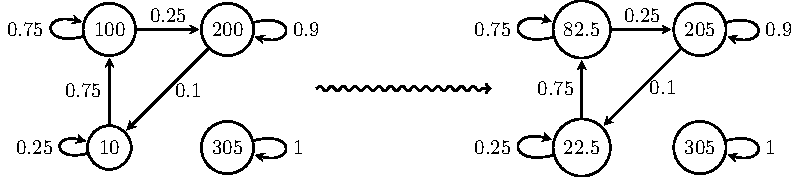
\includegraphics[width=0.9\textwidth]{tikz01}
\caption{The statistical strengths of the first sample before and after the
first time step.}
\end{figure}


\begin{figure}[h]
	\centering
        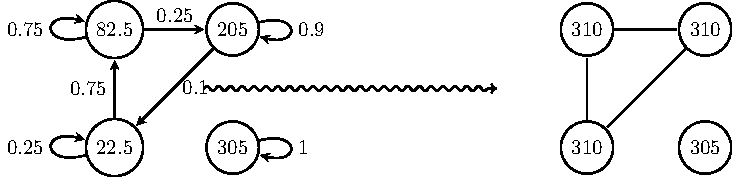
\includegraphics[width=0.9\textwidth]{tikz02}
\caption{Strength of the forces to face at each fort. Note that links are used in both directions.}
\end{figure}
